\documentclass[11pt]{article}
\usepackage{fancyhdr, extramarks, amsmath, amsthm, amsfonts, tikz, algpseudocode, graphicx, tcolorbox}
\usepackage[plain]{algorithm}
\graphicspath {{graphs/}}
\usetikzlibrary{automata,positioning}

\topmargin=-0.45in
\evensidemargin=0in
\oddsidemargin=0in
\textwidth=6.5in
\textheight=9.0in
\headsep=0.25in
\title{\textbf{Introduction to Artificial Intelligence\\
		\large Project 4: Colorization}}
\author{Brenton Bongcaron and Abe Vitangcol\\NetIDs: bdb101 and alv88}
\date{May 5, 2021}
\begin{document}
	\maketitle
\textit{We have read and abided by the rules laid out in Canvas, We have not used anyone else's work for our project, and our work is only our own.}
\tableofcontents
\listoffigures
\pagebreak
\section{Introduction}

Imagine this: you want to send an image to someone, but trying to send the image will cause some error, saying how the image was too large to send. This is commonly seen on applications such as Discord where they limit the size of the images people are allowed to send (unless, with paid perks of course) and the image cannot send. So, instead, the image gets rejected to send unless it has been compressed to lower the size of the image file. So, then the question becomes: how does the image become compressed and the file size becomes lower than the original? The answer: through simplifying the image into similar colors, thus reducing the size. Hence, this project will do such thing, simplifying an image and use less colors to represent the same thing.

\section{The Image}
To test out our algorithms to see how well it does, we have to use a common image and see the algorithm's quality in terms of both representation (how well it represents the original image) and in terms of aesthetics (how appealing it looks to the eye). The image needs to have a balance of colors on both sides and not too much of a color spread. The image we needed was, in fact, the doge, and thus, the doge became the image we tested on.

\begin{figure}[h]
\centering
\includegraphics[scale=1.10]{images/smoldoge.jpg}
\caption{Wow, such beauty, much colors, many fun. Will it go to the moon?}
\end{figure}

\section{The Basic Agent}
To start, the basic agent was necessary as a baseline of how well our advanced algorithm works. The basic agent begins with clustering the colors into 5 best representative colors using k-Nearest Neighbors calculations. Then, the basic agent has 2 arrays, one a grayscale verison of the doge, the other the original image. Using the left half of the grayscale image as training, it replaces 3x3 patches with one of the representative colors accordingly. Then it goes to the right half and tries to fill in the rest of the colors based on what it learned through the training, with a black border around the right half because of how some tiles do not give enough information to complete the image. The result is the following:

\begin{figure}[h]
\begin{minipage}[c]{0.5\textwidth}
\centering
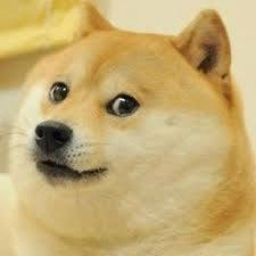
\includegraphics[scale=0.94]{images/smolDoge.jpg}
\begin{center}
Original
\end{center}
\end{minipage}
\begin{minipage}[c]{0.5\textwidth}
\centering
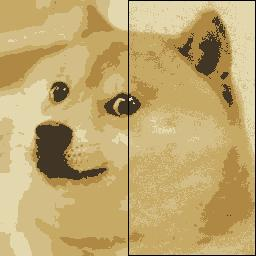
\includegraphics[scale=0.70]{images/basic.jpg}
\begin{center}
Basic Agent
\end{center}
\end{minipage}
\caption{Colors Much, Beauty Such, Woah.}
\end{figure}
\section{The Advanced Agent}
The newest question then becomes: can we create something that beats a 5-Nearest Neighbor calculation and create a better image than the basic agent? The answer was a simple one, there always was a way to beat it, specifically, using logistic regression. We do this using a method called in AI.py, named weightFitting:

\begin{verbatim}
def weightFitting(image):
    im_width, im_height <- image.size
    rgbMatrix <- numpy matrix form of image
    grayIm <- numpy matrix form of grayscale image
    alpha = 0.0001
    wR <- initialization of all weights for "red" model to 0.5
    wG <- initialization of all weights for "blue" model to 0.5
    wB <- initialization of all weights for "green" model to 0.5
    for 150000 rounds of training:
        randPixel <- random pixel on LEFT side of image
        r, g, b <- RGB values of randPixel
        gray = [1]
        for x in range(-1,2):
             for y in range(-1,2):
                  currentPixel <- (randPixel[0]+x, randPixel[1]+y) 
                  gray.append(grayscale value, divded by 255, of currentPixel)
        # Note that dotP() means dot product
        Rx = dotP(wR, gray)
        Gx = dotP(wG, gray)
        Bx = dotP(wB, gray)

        predR = 255.0 / (1 + exp(-1 * Rx))
        Do the above calculation for the other two colors

        gLossR = [(predR - r)*predR*(1 - predR/255.0)*gray[i] for i in range(len(gray))]
        Do the above calculation for the other two colors

        update the weights of the colors' models

    return the weights of the colors' models
\end{verbatim}
Note that the gradient of the loss function is calculated by the formula:
\[
(\text{predicted} - \text{actual})*(\text{predicted})*(1 - \frac{\text{predicted}}{255.0}) * \text{grayscale value}
\]
The predicted color value(for each color) is:
\[
R = \frac{255.0}{(1 - e^{dotP(wR, gray)})}
\]
\[
G = \frac{255.0}{(1 - e^{dotP(wG, gray)})}
\]
\[
B = \frac{255.0}{(1 - e^{dotP(wB, gray)})}
\]
where dotP() denotes dot product.
Note the Color Sum where is says "Rx", "Gx", and "Bx" in the code. After doing all of this, one update is done on all of the weighted values of the colors, which is where we use alpha and the loss values:
\[
(\text{Current Color Weight}) - (\alpha * \text{Gradient of Loss of Color})
\]
This is what is used to update the weights of the colors and is returned after all the trials. Note the alpha and initial weight values seen within the code were found by performing many tests and checking various values before settling on the current values seen. As for the training, more was better since the weights was going converge anyway and the training was fast, so more was done. This concludes the function weightFitting, with the weights of the colors returned to the advanced agent where it uses them to complete the picture.

The result of the Advanced AI is shown in Figure 3.

\begin{figure}[h]
\begin{minipage}[c]{0.5\textwidth}
\centering
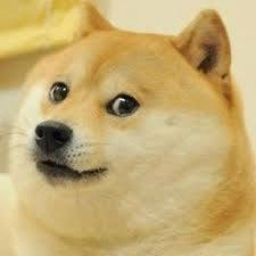
\includegraphics[scale=0.94]{images/smolDoge.jpg}
\begin{center}
Original
\end{center}
\end{minipage}
\begin{minipage}[c]{0.5\textwidth}
\centering
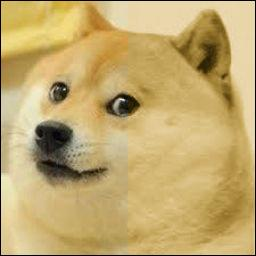
\includegraphics[scale=0.70]{images/advanced.jpg}
\begin{center}
Advanced Agent
\end{center}
\end{minipage}
\caption{Wow, such beauty, much shading, many wows.}
\end{figure}

In terms of quality, it definitely has more colors than the basic agent and, aesthetically speaking, it looks much better than the, err... abstract art doge. The advanced agent colors and shades the doge really well, loses the black border surrounding the right-half of the picture, and, in terms of time, it complete the doge faster than the basic agent. The basic agent takes around 7 minutes to complete its picture whereas the advanced agent took only 30 seconds to a minute to complete with a better quality. Given how both used the same picture and the way both agents completed the doge, it seemed fair to say the basic agent was not as capable as the advanced agent, but both did their jobs well.

However, should there be enough time and resources to complete this (and not a span of two to three weeks because of unfortunate college classes), there would be plans to use neural networks to color the image. There would also be plans to make the algorithm faster (faster than 30 seconds because there is never anything wrong with faster) and test it on more than just doge.

\section{Contributions}
\subsection*{Brenton Bongcaron [bdb101], Section 3}
I did all of the coding of the basic and advanced agents. I also made edits to the \LaTeX\: document.
\subsection*{Abe Vitangcol [alv88], Section 8}
I completed this \LaTeX\: document and did some proofreading and commenting on the code. Wording the \LaTeX\: document was something both my partner and I agreed I liked doing as well as having fun with the doge memes here. Unfortunately, many things came up on my end (mainly affecting my mental health) and thus I wasn't able to work on this project as much as I wanted to. Many apologies to my partner for being unable to help well on this one.
\end{document}